\section{From SMPL to a body-plan-agnostic model}

\term{SMILify} keeps the recipe that made \term{SMPL}~\cite{smpl} and
\term{SMAL}~\cite{smal} useful (a fixed-topology template mesh, deformed by
a low-dimensional shape vector $\bm\beta$ and a per-joint pose $\bm\theta$
under linear blend skinning) and removes the assumption both predecessors
still made: that the skeleton's topology is known and shared in advance
(24 human joints, or a common quadruped rig). SMIL instead accepts an
arbitrary rigged mesh as its template, so the same fitting machinery serves a
six-legged, antenna- and mandible-bearing ant as readily as a mammal.

\begin{figure}[!htb]
\centering
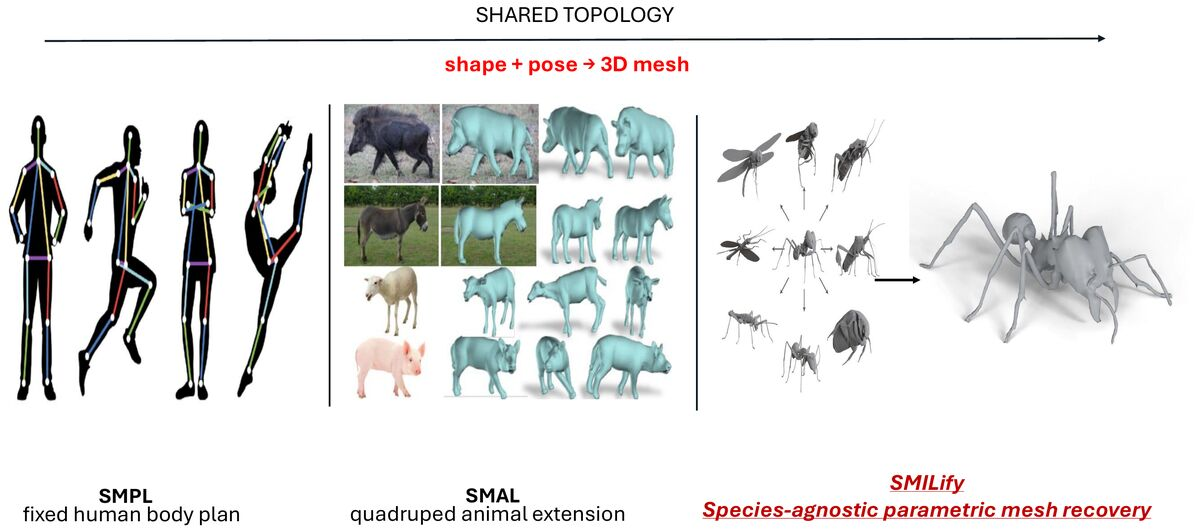
\includegraphics[width=0.62\linewidth]{figures/fig_model_lineage.jpg}
\caption{The lineage of body-plan-agnostic parametric models: a fixed human
topology (SMPL), a shared quadruped rig learned from toy figurines (SMAL),
and \term{SMILify}, which fits an arbitrary rigged template (here an
ant) to scan-derived meshes of any body plan.}
\label{fig:lineage}
\end{figure}

Every fitted specimen is expressed in the same model coordinate system
(Figure~\ref{fig:coord}): the same vertex index always refers to the same
named anatomical locus, so that once a corpus is registered, quantities such
as head width or leg segment length become directly comparable across
specimens without any further alignment step. This is the property the whole
pipeline exists to protect; \S\ref{sec:correspondence-def} makes precise what
can go wrong with it.

\begin{figure}[!htb]
\centering
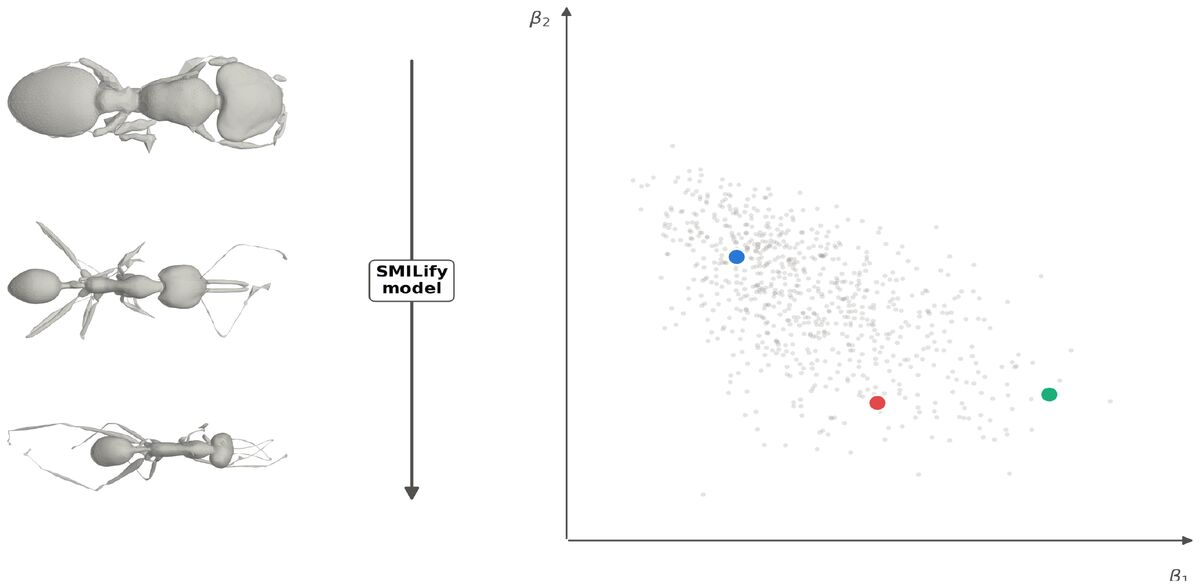
\includegraphics[width=0.62\linewidth]{figures/fig_parameter_space.jpg}
\caption{One shared parameter space, many specimens: the low-dimensional
shape vector $\bm\beta$ learned by the model places every registered
specimen at a point in a common space, in which distance is anatomically
meaningful.}
\label{fig:coord}
\end{figure}
